\documentclass[footmark=none]{tubaf-thesis}
\KOMAoptions{
	listof=totoc,
}
\usepackage[sans]{tubaf-fonts} % Arial
\usepackage[]{tubaf-fonts}    % Times
\usepackage{graphicx}
\usepackage{csquotes}
\usepackage{acronym}
\usepackage{tocbibind}
\usepackage{booktabs}
\usepackage[ngerman]{babel}
\usepackage[backend=bibtex, sorting=none]{biblatex}
\addbibresource{trueRef.bib} % Verknüpfung zur .bib-Datei

\usepackage{chngcntr}
\counterwithout{figure}{chapter}
\counterwithout{table}{chapter}

\usepackage[pdfborderstyle={/S/U/W 1}]{hyperref}

\subject{Seminararbeit}
\title{Energieeffiziente Eingebettete Systeme:\\Dynamische Spannungs- und Frequenzskalierung}
\author{Ben Weckend\\{\small Matrikel: 67551}}
\date{30. August 2024}
\examiners{Prof. Dr. Bernhard Jung \and M.Sc. Robert Lösch}
\course{Diplom Robotik}

% Document
\begin{document}

    \pagenumbering{roman}

    \maketitle
    \makedeclarationofauthorship[30. August 2024]
    \tableofcontents
    
    \newpage
    \listoffigures 						% Abbildungsverzeichnis
    \newpage
    \listoftables 						% Tabellenverzeichnis
    
    \newpage
    \chapter*{Abkürzungsverzeichnis}
    \addcontentsline{toc}{chapter}{Abkürzungsverzeichnis}
    \begin{acronym}[EPROM]  % Längste Abkürzung hier angeben, um die Ausrichtung zu verbessern
    	\acro{AISC}{Application-Specific Integrated Circuit (anwendungsspezifische integrierte Schaltung)}
    	\acro{CPU}{Central Processing Unit (Zentrale Verarbeitungseinheit eines Computers)}
    	\acro{CIL}{Current Interval Length (aktuelle Intervalllänge)}
    	\acro{TIL}{Target Interval Length (erzielte Zielintervalllänge)}
    	\acro{DVFS}{Dynamic Voltage and Frequency Scaling (Technik zur dynamischen Anpassung von Spannung und Frequenz zur Energieeinsparung)}
    	\acro{EPROM}{Erasable Programmable Read-Only Memory (löschbarer programmierbarer Nur-Lese-Speicher)}
    	\acro{ROM}{Read-Only Memory (Nur-Lese-Speicher, ein nicht flüchtiger Speicher)}
    	\acro{FPGA}{Field-Programmable Gate Array (feldprogrammierbares Gatter-Array, eine Art integrierter Schaltkreis)}
    	\acro{GPU}{Graphics Processing Unit (Grafikprozessor, zuständig für die Bildberechnung)}
    	\acro{MTBF}{Mean Time Between Failures (mittlere Betriebsdauer zwischen Ausfällen, eine Zuverlässigkeitskennzahl)}
    	\acro{PCB}{Printed Circuit Board (Leiterplatte, auf der elektronische Bauteile montiert werden)}
    \end{acronym}
    
    \clearpage
    \pagenumbering{arabic}
    
    \chapter{Einleitung}
    	Energieeffizienz ist seit jeher ein zentrales Thema in der Technologieentwicklung. Das Ziel, möglichst viel Energie zu erzeugen und gleichzeitig den Verbrauch zu minimieren, bleibt unverändert – dabei soll der Komfort nicht eingeschränkt und Kosten gesenkt werden. In einer zunehmend vernetzten Welt mit hohen Anforderungen an Leistung und Flexibilität wird eine effiziente Energienutzung immer wichtiger \cite{hintemann2016trotz}. Gerade in eingebetteten Systemen, die mobil und langlebig sein müssen, ist dies essenziell. Dynamische Spannungs- und Frequenzskalierung (DVFS) bietet hier eine Lösung, indem sie den Energieverbrauch in Echtzeit an die Lastanforderungen anpasst.
    	\section{Hintergrund und Motivation}
   			Moderne integrierte Systeme müssen hohe Leistung bei langer Betriebsdauer gewährleisten. Besonders in tragbaren oder implantierbaren medizinischen Geräten, wie für eine Langzeit-Holter-Überwachung, ist Energieeffizienz entscheidend. Diese Systeme müssen leicht, unauffällig und über lange Zeit zuverlässig funktionieren, ohne häufigen Batteriewechsel. Gleichzeitig müssen sie komplexe Kommunikationsprozesse und die Überwachung wechselnder Variablen meistern. Die Dynamische Spannungs- und Frequenzskalierung (DVFS) bietet hier eine Lösung, indem sie den Energieverbrauch durch Anpassung der Prozessorleistung an die Anforderungen optimiert. \cite{5256133}
    	\section{Struktur und Zielsetzung der Arbeit}
    		Die Arbeit behandelt zunächst die Grundlagen eingebetteter Systeme und deren Energieeinsparpotenzial durch ein passendes AICS-Design. Anschließend wird der Effekt der Dynamischen Spannungs- und Frequenzskalierung (DVFS) sowie die Auswahl geeigneter Echtzeitanwendungen erläutert. Der Fokus liegt auf der Frequenz- und Spannungsskalierung, gefolgt von ergänzenden Stromsparmechanismen wie Power Gating, Clock Gating und Sleep-Modi. Abschließend werden Fallstudien und zukünftige Entwicklungen von DVFS diskutiert.
    		 Ziel dieser Arbeit ist es, die Vorteile und Herausforderungen von DVFS zur Verbesserung der Energieeffizienz in eingebetteten Systemen zu analysieren.
    
    \chapter{Grundlagen}
    	\section{Eingebettete Systeme und deren Anwendungen}
    		Eingebettete Systeme sind aus unserer modernen Welt nicht mehr wegzudenken. Sie finden sich in nahezu allen Bereichen des täglichen Lebens – von Luft- und Raumfahrttechnik über Automobile bis hin zu Alltagsgegenständen wie Uhren. Besonders im Automobilbereich spielen sie eine zentrale Rolle: In etwa 40\% der Kosten eines Neuwagen fallen auf Elektronik und Software, während 90\% der technologischen Innovationen in diesem Sektor auf diese Bereiche zurückzuführen sind. \cite{berns2010eingebettete}
    		
    		Ein eingebettetes System ist ein spezialisiertes Computersystem, das aus einer Kombination von Hardware und Software besteht und für eine spezifische Funktion entwickelt wurde. Diese Systeme, oft basierend auf Mikroprozessoren oder FPGAs, sind in größere Systeme integriert und übernehmen dort meist unsichtbar wichtige Aufgaben. Im Gegensatz zu herkömmlichen Computern verfügen sie häufig über keine Benutzeroberfläche und arbeiten autonom im Hintergrund. Sie steuern spezifische Funktionen in Echtzeit und müssen dabei strengen Anforderungen an Kosten, Energieverbrauch und Größe gerecht werden, dazu aber auch präzise auf Umweltveränderungen reagieren können um eine bestimmte Aufgabe kontinuierlich und zuverlässig auszuführen. \cite{gessler2014entwicklung}
    	\section{Energieeffizienz in eingebetteten Systemen}
    		Eingebettete Systeme bestehen typischerweise aus einem Prozessor, Speicher, einer Stromversorgung und Kommunikationsports. Die Auswahl der Komponenten ist entscheidend für die Effizienz und Funktionalität des Systems. Ein wichtiges Beispiel ist die Entscheidung zwischen verschiedenen Speichertypen: ROM (Read-Only Memory) und EPROM (Erasable Programmable Read-Only Memory). ROM, als Festwert- oder Nur-Lese-Speicher, ist nichtflüchtig und bietet schnellen Zugriff, kann jedoch im Betrieb nicht überschrieben werden. EPROM hingegen ermöglicht ebenfalls nichtflüchtige Speicherung, ist jedoch langsamer als ROM. \cite{klar2015integrierte}
    		
    		Auch die Wahl zwischen Mikroprozessoren oder Mikrocontroller kann die Energieeffizienz beeinflussen. Der Prozessor in einem eingebetteten System kann ein Mikrocontroller oder ein Mikroprozessor sein. Der Unterschied zwischen diesen Komponenten besteht darin, dass Mikroprozessoren mehr Unterstützungsschaltungen benötigen, da der Speicher und die Peripherie nicht auf dem Chip enthalten sind und stattdessen separate integrierte Schaltkreise verwendet werden. Mikrocontroller hingegen haben diese auf dem Chip integriert.  Ein Vorteil eines Mikroprozessors ist die Möglichkeit, die Systemfunktionen auf das Wesentliche zu beschränken und nur genau die benötigten Komponenten zu integrieren, was eine gezielte Optimierung ermöglicht. \cite{Urbanski2004}
    		\subsection{ASIC Design}
    			Eine gezielte Optimierung führt zu einem weiteren wichtigem Ansatz zur Steigerung der Energieeffizienz in eingebetteten Systemen: die Verwendung von anwendungsspezifischen integrierten Schaltungen ('Application-Specific Integrated Circuit' (ASICs)). Im Gegensatz zu generischen Mikroprozessoren oder Mikrocontrollern sind ASICs speziell für eine bestimmte Anwendung entworfen und optimiert. Dadurch können unnötige Funktionen und Schaltungen vermieden werden, was zu einer deutlichen Reduzierung von Energieverbrauch, Platzbedarf und Kosten führt. Da ein ASIC exakt auf die spezifischen Anforderungen einer Aufgabe zugeschnitten ist, kann die Effizienz sowohl in Bezug auf Rechenleistung als auch Energieverbrauch maximiert werden und die Geschwindigkeit, den Stromverbrauch und die Verzögerung des ASIC-Chips deutlich verbessert werden. \cite{10.1145/337292.337604} \cite{Matiieshyn2023} 
    			
    			Allerdings ist die Entwicklung eines ASICs mit höheren initialen Entwicklungs- und Herstellungskosten verbunden, weshalb sich dieser Ansatz hauptsächlich in Anwendungen mit hohen Stückzahlen oder besonderen Leistungsanforderungen lohnt, wie etwa in der Automobilindustrie oder bei medizinischen Geräten. Die präzise Abstimmung der Schaltungsarchitektur auf die Zielanwendung macht ASICs besonders geeignet für energieeffiziente eingebettete Systeme, bei denen langfristige Zuverlässigkeit und niedriger Energieverbrauch entscheidend sind. \cite{Matiieshyn2023}
    			
    			Während die Auswahl der richtigen Komponenten und die Verwendung spezialisierter Schaltungen wie ASICs wichtige Schritte zur Optimierung der Energieeffizienz darstellen, reichen diese Ansätze allein oft nicht aus, um die Anforderungen moderner, hochdynamischer Systeme zu erfüllen. Insbesondere in Anwendungen, bei denen die Lastbedingungen stark schwanken, ist eine flexible Anpassung der Leistungsaufnahme entscheidend. Hier kommt die Dynamische Spannungs- und Frequenzskalierung (DVFS) ins Spiel, die eine adaptive Steuerung der Systemressourcen in Echtzeit ermöglicht.
    	\section{Dynamische Spannungs- und Frequenzskalierung Konzepte und Prinzipien}
    		DVFS ist eine Technik, bei der die CPU-Frequenzen und -Spannungen automatisch an die aktuelle Systemlast angepasst werden. Bei niedriger Arbeitsbelastung reduziert das System die Spannung und Frequenz, um Energie zu sparen, während bei hoher Last die Spannung und Frequenz erhöht werden, um die Leistung zu maximieren \cite{5545490}. Diese dynamische Anpassung bringt mehrere direkte Vorteile: Durch eine verbesserten Zuverlässigkeit und einer längeren Produktlebensdauer können auch bessere MTBF-Werte (Mean Time Between Failures) erreicht werden. Zudem wird durch die optimierte Stromversorgung das Rauschen in den Schaltkreisen reduziert, was zu effizienteren Spannungsreglern und durch sparsames schalten der Transistoren zu weniger Wärmeentwicklung führt. \cite{9441002}
    		
    		Ein wesentlicher Bestandteil von DVFS ist die Steuerlogik, die kontinuierlich die aktuelle Systemlast überwacht und in Echtzeit entsprechende Anpassungen vornimmt. Diese Anpassungen basieren auf Parametern wie der CPU-Auslastung, Temperatur und den geforderten Leistungsanforderungen. Als erstes wird eine Leistungsanalyse durchgeführt, um zu bestimmen, welche Frequenz- und Spannungseinstellungen in unterschiedlichen Lastsituationen optimal sind.
    		
    		Dabei gilt es zu beachten, dass eine Erhöhung der Frequenz auch eine höhere Spannung erfordert, um die neue Leistung der Schaltung zu ermöglichen. Dies sieht man gut an der Frequenz und Betriebsspannung der dem Intel Pentium M Prozessor (\autoref{IntelPentM}) aus dem Jahr 2003. \cite{khabi2018energieeffizienz} 
    		
    		\begin{table}[!ht]
    			\centering
    			\begin{tabular}{l|r}
    				$GHz$ & $V_{CC}$ \\ \hline
    				$1.6$ & $1.484$ \\
    				$1.4$ & $1.420$ \\
    				$1.2$ & $1.276$ \\
    				$1.0$ & $1.164$ \\
    				$0.8$ & $1.036$ \\
    				$0.6$ & $0.956$
    			\end{tabular}
    			\caption{CPU-Frequenz und Betriebsspannung des Intel Pentium M Prozessors \cite{khabi2018energieeffizienz}}
    			\label{IntelPentM}
    		\end{table}
    		
    		 Dies führt zu einer erhöhten Leistung, aber auch zu einem stetig ansteigenden Energieverbrauch, weshalb aus diesem Grund die Steuerlogik die Spannungserhöhung nur dann optimiert, wenn es tatsächlich notwendig ist.
    		\subsection{Wählen der richtigen Echtzeitapplikation}
    			Bei der Anwendung von DVFS wird die Spannung und Frequenz dynamisch an die aktuelle Last angepasst. Dieser Prozess benötigt jedoch eine gewisse Reaktionszeit, während der das System möglicherweise nicht in der Lage ist, seine Fristen vollständig einzuhalten (Siehe \autoref{chap:Frequenzskalierung}) .Die Auswirkungen dieser Verzögerung können je nach Art der Echtzeitapplikation erheblich variieren, weshalb eine genaue Analyse der Anwendungsanforderungen vor der Integration von DVFS entscheidend ist. Grundsätzlich lassen sich Echtzeitsysteme in drei Typen unterteilen: harte, feste und weiche Echtzeitapplikationen.
    			
    			\textbf{Harte Echtzeitapplikationen}zeichnen sich dadurch aus, dass eine verpasste Deadline zu einem vollständigen Systemausfall führen kann. In sicherheitskritischen Bereichen wie der Medizintechnik oder dem Automobilsektor können solche Verspätungen katastrophale Folgen haben. Hier ist die Implementierung von DVFS besonders kritisch, da selbst geringfügige Verzögerungen in der Anpassung von Spannung und Frequenz das gesamte System gefährden könnten. Trotz dessen sind harte Echtzeitsysteme legitim solange das System konstante Leistungsanforderungen hat. \cite{scholz2005softwareentwicklung}
    			
    			\textbf{Feste Echtzeitapplikationen} sind weniger strikt, da das Verpassen einer Deadline keinen direkten Schaden verursacht. Allerdings wird der Fortschritt der Berechnung in solchen Fällen verworfen, da die Ergebnisse nach Ablauf der Frist als unbrauchbar betrachtet werden. Ein Beispiel hierfür wäre die Verarbeitung von Videodaten, bei der verspätete Frames einfach übersprungen werden, um die Synchronität zu wahren. \cite{scholz2005softwareentwicklung}
    			
    			\textbf{Weiche Echtzeitapplikationen} bieten die größte Flexibilität, da sie kleinere Verzögerungen tolerieren können, ohne dass dies zu schwerwiegenden Fehlern führt. Hier können auch unvollständige Berechnungen nützlich sein, da Teilergebnisse oft durch Interpolations- oder Schätzungsverfahren ergänzt werden können. In einigen Fällen kann die Berechnung sogar zu einem späteren Zeitpunkt fortgesetzt werden. Aufgrund dieser Toleranzgrenze eignen sich weiche Echtzeitapplikationen besser für DVFS, da die potenziellen Auswirkungen von Totzeiten und Anpassungsverzögerungen weniger kritisch sind. \cite{scholz2005softwareentwicklung}
    			
    			Mit dem Verständnis von Echtzeitsystemen kann nun die Frequenz in einer weichen Echtzeitapplikation so eingestellt werden, dass sie gerade ausreicht, um die Arbeitslast rechtzeitig abzuschließen: idealerweise kurz bevor die nächste Arbeitslast eintrifft \cite{5545490} \cite{5256133}. Diese Strategie zielt darauf ab, die Anzahl der Leerlaufzyklen zu minimieren, in denen der Prozessor unnötig Energie verbraucht, also ohne signifikante Arbeit zu leisten. Dadurch kann zwar Energie gespart werden, allerdings leidet die Effizienz, besonders in leistungskritischen Momenten erheblich. Um eine hohe Effizienz sicherzustellen, muss die bereitgestellte Leistung dynamisch an die tatsächlichen Anforderungen angepasst werden.
    
    \chapter{Technik zur Dynamischen Spannungs- und Frequenzskalierung}
    
    	\section{Frequenzskalierung}
    	\label{chap:Aktivitätsmonitor}
    		Bei der Spannungsskalierung spielt die Frequenzplanung eine entscheidende Rolle, insbesondere in Verbindung mit einem Aktivitätsmonitor. Der Aktivitätsmonitor überwacht die Anzahl der Leerlaufzyklen des Prozessors während der Laufzeit, um in festen Aktualisierungsintervallen die Auslastung und Effizienz des Systems zu analysieren, woraufhin basierend die Frequenz dynamisch an die aktuelle Arbeitslast angepasst wird. \cite{1374987}
    		\subsection{Frequenzaktualisierungsintervalle}
    		Die Frequenzaktualisierungsrate des Monitors ist direkt mit der Grundtaktfrequenz des Prozessors verknüpft. Größere Intervalle führen zu weniger häufigen Frequenzänderungen und erschweren es, auf Veränderungen der Arbeitslast schnell zu reagieren. Im Gegensatz dazu bewirken kleinere Intervalle häufigere Aktualisierungen, was jedoch zu unnötigen Anpassungen und somit zu einer instabilen Systemleistung führen kann. Die Wahl des richtigen Aktualisierungsintervalls ist daher ein Balanceakt zwischen Reaktionsfähigkeit und Stabilität. \cite{5545490} \cite{4110118}
    		\subsection{Dynamische Skalierung}
    		\label{chap:Frequenzskalierung}
    		Während der Ausführung einer Arbeitslast zählt ein Zykluszähler die Systemtaktzyklen und bestimmt die aktuelle Intervalllänge (CIL). Diese wird mit einer vorab definierten Zielintervalllänge (TIL) verglichen. Wenn die CIL kürzer ist als die TIL, wird die Zielintervalllänge in kleinen Schritten verringert (siehe \autoref{fig:screenshot001}(a)), was darauf hindeutet, dass die aktuelle Frequenz zu hoch ist und abgesenkt werden kann. Wenn die Arbeitslast jedoch länger dauert und die CIL die TIL überschreitet (siehe \autoref{fig:screenshot001}(b)), kann der Workload nicht beendet werden, woraufhin die Zielintervalllänge erhöht wird, um die Frequenz anzupassen und die Berechnungsleistung zu steigern. \cite{5545490}
    		
    		\begin{figure}[!ht]
    			\centering
    			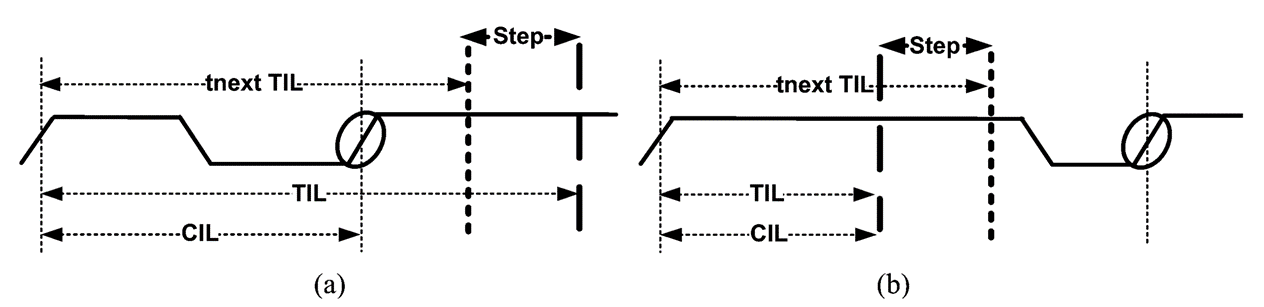
\includegraphics[width=0.9\linewidth]{img/screenshot001}
    			\caption{Effektives Konzept der Fristenvorhersage für Fälle, die (a) einer Intervallverringerung und (b) einer Intervallvergrößerung entsprechen. \cite{5545490}}
    			\label{fig:screenshot001}
    		\end{figure}
    		
    		Der Schlüssel zur Effizienz dieses Ansatzes liegt in der adaptiven Anpassung des Intervallschritts. Wenn mehrmals in Folge eine Erhöhung oder Verringerung der TIL erforderlich ist, wird der Intervallschritt verdoppelt oder halbiert, um auf starke Veränderungen in der Arbeitslast reagieren zu können. Dieser Mechanismus vermeidet unerwünschte und unnötige Frequenzanpassungen und sorgt gleichzeitig dafür, dass abrupte Veränderungen der Arbeitslast schnell und präzise verfolgt werden. \cite{5545490}
    		
    		Ein Vorteil dieses adaptiven Frequenzplanungsalgorithmus ist, dass er sich dynamisch an Veränderungen der Arbeitslast anpasst. Besonders in weichen Echtzeitsystemen kann diese Flexibilität genutzt werden, um den Energieverbrauch zu minimieren, ohne die Gesamtleistung erheblich zu beeinträchtigen. Selbst bei temporären Verzögerungen bleibt das System stabil. Der Nachteil liegt jedoch in der Reaktionsverzögerung bei plötzlichen Lastwechseln. In einem 'Overloaded State' kommt es zu einem sehr schnellen Anstieg an Workload woraufhin die Frequenzanpassung zu langsam erfolgt, während sie in einem 'Underloaded State' unnötig hoch bleibt, aufgrund einer sehr schnellen Abnahme an Workload, was auf zu geringe Aktualisierungsintervalle zurückgeführt werden kann. \cite{4110118} \cite{5545490}
    	\section{Spannungsskalierung}
    		Die Kontrolle der Spannung spielt im DVFS-Prozess eine zentrale Rolle, da eine Reduktion der Frequenz ohne entsprechende Anpassung der Spannung nur begrenzte Energieeinsparungen erzielen würde. Zudem kann eine erhöhte Leistung und damit eine höhere Frequenz nur dann realisiert werden, wenn die Spannung entsprechend skaliert wird (Siehe Bsp.: \autoref{IntelPentM}).
    	
    		Allein durch die Frequenzanpassung und eine konstant hohe Spannung ließe sich zwar ein gewisser Stromverbrauch einsparen, allerdings müssen dafür dynamische und statische Leistung differenziert betrachtet werden.
    	
    		\begin{description}
    			\item[Dynamische Leistung] entsteht durch das Schalten der Transistoren, also den Wechsel zwischen Zuständen, und ist unmittelbar von der Frequenz abhängig.
    			\item[Statische Leistung] hingegen fällt bereits an, sobald ein Transistor eingeschaltet ist, unabhängig von dessen Arbeitsaktivität. Sie ist in der Regel niedriger als die dynamische Leistung, verursacht jedoch Energieverluste und sollte vermieden werden \cite{klar2015integrierte}.
    		\end{description}

    		Mit steigender Frequenz nimmt also die dynamische Leistung zu, während die statische Leistung abnimmt. Auf einen gegebenen Zeitintervall bezogen wird bei höherer dynamischer Leistung zwar mehr Energie verbraucht, doch die schnellere Verarbeitung der Workload ermöglicht Einsparungen über den gesamten Arbeitszyklus hinweg. Obwohl es paradox erscheint,  ist es theoretisch somit möglich Energie sparen indem die Frequenz erhöht wird.
    	
    		Dennoch bleibt dies unzureichend, da der Energieverbrauch und somit auch die Leistungsaufnahme eines Halbleiters stark von der Betriebsspannung abhängig sind. Nach der vereinfachten Formel \cite{inbook}:
    		\[P \propto V^2 \cdot f\] 
    		ist die Leistungsaufnahme ($P$) eines Prozessors proportional zum Quadrat der Betriebsspannung ($V$) und zur Taktfrequenz ($f$). Diese Abhängigkeit verdeutlicht, warum selbst geringfügige Anpassungen der Spannung signifikante Auswirkungen auf den Energieverbrauch haben können. Die Gate- und parasitären Kapazitäten sowie Leckströme tragen ebenfalls zur Gesamtleistung bei, was den Energieaufwand weiter beeinflusst. \cite{inbook}
        
      	 	Die Anpassung der Spannung erfolgt basierend auf den Intervallschritten, die aus der Frequenzplanung abgeleitet werden. Diese Informationen werden an die Power Control Unit (PCU) weitergeleitet, die die Spannung entsprechend der aktuellen Arbeitslast reguliert \cite{khabi2018energieeffizienz}. Diese Arbeitslast wird durch den Aktivitätsmonitor überwacht, der sowohl für die Frequenz- als auch für die Spannungsskallierung ausschlaggebend ist (Siehe \autoref{chap:Aktivitätsmonitor}).
        
      	 	Somit werden mehrere wesentliche Vorteile erreicht: durch die Erhöhung der Spannung lässt sich die Taktfrequenz anheben, was eine schnellere Datenverarbeitung und damit eine insgesamt höhere Verarbeitungsgeschwindigkeit ermöglicht. Zudem wird die Leistungsfähigkeit des Systems verbessert, da es in der Lage ist, komplexere Aufgaben und anspruchsvollere Algorithmen effizienter zu bewältigen.
        
			Den Vorteilen stehen jedoch einige Nachteile gegenüber. Eine höhere Leistung führt unweigerlich zu einem gesteigerten Energieverbrauch, was die Effizienz reduzieren kann. Zudem bringt die erhöhte Spannung eine verstärkte Wärmeentwicklung mit sich, die nicht nur die Lebensdauer des Prozessors beeinträchtigen kann, sondern auch den Einsatz einer zusätzlicher Kühlfunktion erforderlich macht.
       	
	\chapter{Grundlegenden Stromspar-Mechanismen}
		
		Effiziente Energieverwaltung ist entscheidend für die Gestaltung eingebetteter Systeme. Neben DVFS gibt es mehrere zusätzliche Techniken, die den Energieverbrauch weiter senken können. Diese Methoden konzentrieren sich auf die Architektur des Systems sowie auf gezielte Mechanismen zur Abschaltung oder Drosselung von Systemkomponenten.
		
		\section{Power Gating und Clock Gating}
			\textbf{Power Gating} schaltet mithilfe von Transistoren gezielt inaktive Teile des Prozessors komplett ab, um Leckströme deutlich zu minimieren. Diese Technik ist besonders effektiv, wenn bestimmte Schaltungsteile über längere Zeit inaktiv bleiben, wodurch erhebliche Energieeinsparungen erzielt werden. Der Einsatz von Power Gating bietet daher signifikante Vorteile bei längerem Stillstand von Systemkomponenten. \cite{1198683}
		
			\textbf{Clock Gating} deaktiviert das Taktsignal für gezielt ausgewählte, ungenutzte Schaltungsbereiche, um den dynamischen Energieverbrauch gezielt zu senken. Ohne aktives Taktsignal finden in diesen Bereichen keine unnötigen Schaltvorgänge statt, wodurch der Energieverbrauch drastisch sinkt. Allerdings bleiben die Leckströme als einzige verbleibende Energiequelle weiterhin bestehen. \cite{1198683}
		
			Clock Gating und Power Gating bieten unterschiedliche Vorteile, abhängig von der gewünschten Granularität und Reaktionszeit \cite{1198683} \cite{F2}:
			
			\begin{description}
				\item[Clock Gating] ermöglicht eine feinere Steuerung auf Ebene einzelner Register oder Flip-Flops und bietet eine schnelle Reaktivierung. Diese Methode eignet sich besonders, wenn kurze Schlafphasen vorgesehen sind und schnelle Reaktionszeiten erforderlich sind.
				\item[Power Gating] \sloppy ist komplexer und erfordert eine Mindestgröße der abzuschaltenden Schaltungsteile, um effizient zu sein. Die Reaktivierung dauert länger, da die Stromversorgung erst wiederhergestellt werden muss. Es eignet sich daher besser für längere Inaktivitätsphasen.
			\end{description}
			
			Eine Kombination beider Techniken kann in vielen Szenarien die besten Energieeinsparungen erzielen.
		
		\section{Cache-Hierarchien optimieren}
			Die Cache-Organisation spielt eine wesentliche Rolle beim Energiemanagement. Durch die Optimierung der Größe und Anordnung von Caches kann der Energieverbrauch erheblich reduziert werden. Indem der Zugriff auf den externen Speicher minimiert wird, reduziert sich nicht nur die Energie, die für den Speicherzugriff benötigt wird, sondern auch die Gesamtleistung wird verbessert, da häufig benötigte Daten schneller bereitgestellt werden. \cite{F1}
		
		\section{Sleepmodus}
			Moderne Mikrocontroller bieten verschiedene vorgefertigte Schlafmodi, die auf unterschiedliche Energiesparanforderungen abgestimmt sind. Die Auswahl des geeigneten Schlafmodus hängt von den Anforderungen der Anwendung ab, insbesondere in Bezug auf Reaktionszeit und Energieeinsparung. Es gibt grundsätzlich drei Hauptmodi:
		
			\begin{description}
				\item[Idle-Modus:] Der CPU-Kern bleibt aktiv, während Peripheriegeräte in den Ruhezustand versetzt werden. Dies ermöglicht eine schnelle Reaktivierung bei minimalem Energieverbrauch. \cite{dermikrocontroller}
				\item[Standby-Modus:] \sloppy Sowohl der CPU-Kern als auch die Peripheriegeräte werden in einen niedrigen Energiezustand versetzt. Dieser Modus bietet einen guten Kompromiss zwischen Energieeinsparung und Reaktivierungszeit, da das System schnell durch externe Ereignisse geweckt werden kann. \cite{dermikrocontroller}
				\item[Power-Down-Modus:] In diesem Modus wird der Mikrocontroller fast vollständig abgeschaltet, wobei nur einige wenige Schaltungen aktiv bleiben, um externe Signale zu überwachen. Dieser Modus bietet maximale Energieeinsparung, allerdings auf Kosten einer längeren Reaktivierungszeit. \cite{dermikrocontroller}
			\end{description}
			
		\section{Energieeffizienz beim PCB-Design}
			Energieeffizienz im PCB-Design ist ein zentraler Faktor bei der Entwicklung von Anwendungen, die auf geringen Stromverbrauch angewiesen sind. Es gibt mehrere Ansätze, um die Energieeffizienz zu maximieren:
		
			Wichtige Maßnahmen umfassen den Einsatz stromsparender Mikrocontroller und Sensoren, die besonders in Standby- und Schlafmodi wirksam sind. Eine optimierte Layout- und Routing-Strategie mit kurzen Leiterbahnen und gezielter Bauteilplatzierung minimiert parasitäre Effekte. Zudem ist die Wahl eines geeigneten Spannungsreglers entscheidend, um eine präzise und stabile Versorgung der Komponenten sicherzustellen.
		
	\chapter{Anwendungen und Fallstudie}
       	
        \section{Fallstudie: DVFS und Grafikkarten}
        	In einer Fallstudie \cite{stachowski2022untersuchung}, die im Rahmen einer Dissertation von Matthias Markus Stachowski an der Universität Bayreuth durchgeführt wurde, ist die Wirksamkeit von DVFS in der Energieoptimierung von Prozessoren untersucht worden. Die Arbeit trägt den Titel \textit{'Untersuchung und Modellierung des Energieverbrauchs von DVFS Prozessoren auf Basis von parallelen Berechnungen des wissenschaftlichen Rechnens'} und fokussiert sich dabei auf den Einsatz von DVFS zur Senkung des Energieverbrauchs bei GPUs.
        	
        	In der Studie wurde ein Autotuning-Framework eingesetzt, das die Energieeffizienz von NVIDIA-GPUs durch dynamische Anpassung von Frequenz und Spannung optimiert. Der Autotuner erlaubt es, mehrere GPUs eines Systems gleichzeitig zu nutzen und die optimale Energieeinstellung über verschiedene Suchstrategien zu ermitteln. Als Anwendungsfall wurde das energieintensive Kryptomining gewählt, bei dem das Framework darauf abzielte, den Energieverbrauch zu minimieren, ohne signifikante Leistungseinbußen hinzunehmen.
        	
        	Das Framework wurde mit verschiedenen Grafikkarten und Kryptowährungen getestet, wobei sich deutliche Effizienzsteigerungen zeigten. Je nach Kombination von Grafikkarte und Kryptowährung konnte eine Steigerung der Energieeffizienz von bis zu 84\% erreicht werden. Diese Ergebnisse bestätigen die Wirksamkeit von DVFS in der Praxis und betonen ihr Potenzial. Die Arbeit von Stachowski verdeutlicht, wie durch eine gezielte Anpassung der Betriebsparameter Einsparungen erzielt werden können, was insbesondere in Szenarien mit hohem Energiebedarf von großer Bedeutung ist.
         
        \section{DVFS in mobilen Geräten, Weltraumtechnik und Sonden}
        	In der Weltraumtechnik, insbesondere bei Sonden und Satelliten, könnte DVFS eine entscheidende Rolle für die Energieeffizienz spielen. Da die Energieversorgung im All begrenzt ist, ermöglicht DVFS, die Leistung dynamisch anzupassen und so den Energieverbrauch zu minimieren. Bei kritischen Manövern oder datenintensiven Operationen kann die Leistung gesteigert werden, während sie in Phasen der Inaktivität stark reduziert wird, um Ressourcen zu schonen und die Betriebsdauer zu maximieren.
        
        
        
	\chapter{Schlussfolgerung}
        
       	Die Energieeffizienz steht im Mittelpunkt der technologischen Entwicklung. In einer zunehmend vernetzten und mobilen Welt, in der Geräte kleiner und leistungsfähiger werden, ist es entscheidend, den Energieverbrauch zu minimieren, ohne die Leistung oder den Komfort zu beeinträchtigen. Vor allem in eingebetteten Systemen, wie tragbaren medizinischen Geräten, ist Energieeffizienz essenziell. Hier bietet die DVFS eine flexible Lösung, indem sie die Prozessorleistung in Echtzeit an die aktuellen Anforderungen anpasst.
    		
    	\section{Ausblick auf zukünftige Forschungsrichtungen und Herausforderungen}
    		Die Zukunft der dynamischen Spannungs- und Frequenzskalierung (DVFS) wird stark durch die zunehmende Komplexität moderner Systeme bestimmt. Zwei Trends werden sich dabei höchst wahrscheinlich abzeichnen: eine feinere Granularität und der verstärkte Einsatz heterogener Systeme.
    		
    		\begin{description}
    			\item[Feinere Granularität:] Traditionell wurde DVFS auf Ebene des gesamten Prozessors oder einzelner Kerne eingesetzt. Zukünftig wird jedoch eine feinere Granularität angestrebt, bei der Spannungs- und Frequenzanpassungen auf noch kleinere Einheiten, wie einzelne Funktionsblöcke oder sogar Transistoren, angewendet werden. Diese präzisere Steuerung ermöglicht eine noch effizientere Energienutzung. Eine Herausforderung dabei ist die Koordination dieser kleineren Einheiten ohne erhebliche Overheads, die den Energieeinsparungen entgegenwirken könnten.
    			\item[Heterogene Systeme:] Heutige Chips setzen immer mehr auf eine Mischung aus verschiedenen Prozessortypen. In solchen Systemen wird DVFS dann richtig spannend: Man passt nicht nur die Spannung und Frequenz an, sondern wechselt auch dynamisch zwischen den unterschiedlichen Kernen, je nach dem, was die aktuelle Aufgabe braucht. Das heißt, der Chip entscheidet, ob für eine Aufgabe eher der schnelle oder der sparsame Kern genutzt wird. Die Kunst liegt darin, das alles clever zu steuern, ohne dass es zu kompliziert wird.
    		\end{description}
    		
    	In Zukunft wird DVFS also noch präziser und flexibler. Gleichzeitig müssen all diese Steuermechanismen in immer komplexere, heterogene Systeme integriert werden. Das Ziel bleibt, die Leistung und Energieeffizienz optimal auszubalancieren
    	
    \chapter{Zusammenfassung eines anderen Seminarvortrags}
    	
    		{\Large \textbf{Einsatzmöglichkeiten von FPGAs in der Robotik: Überblick über die Technologie am Beispiel der Anwendung in Weltraumrobotern}} \\
    	
   			FPGAs (Field-Programmable Gate Arrays) spielen eine bedeutende Rolle in der Robotik, insbesondere in anspruchsvollen Anwendungen wie Weltraumrobotern. Diese programmierbaren Schaltungen bieten eine flexible Hardware, die nach Bedarf konfiguriert werden kann. Im Gegensatz zu Mikroprozessoren können FPGAs parallel arbeiten und sind daher ideal für Aufgaben, die hohe Rechenleistung und Echtzeitverarbeitung erfordern.
   			
   			\textbf{Grundprinzipien:} FPGAs bestehen aus Logikgattern, die vom Nutzer konfiguriert werden können, um spezifische Aufgaben direkt in Hardware abzubilden. Durch ihre parallele Architektur sind sie in der Lage, mehrere Aufgaben gleichzeitig zu erledigen, was zu höherer Effizienz und geringerem Energieverbrauch führt. Daraus ergeben sich mehrere Hauptvorteile:
    
			\begin{description}
				\item[Echtzeitverarbeitung:] In Weltraumrobotern müssen Daten in Echtzeit verarbeitet werden. FPGAs ermöglichen eine schnelle Reaktionsfähigkeit auf externe Signale.
				\item[Flexibilität:] Da die Anforderungen bei Weltraummissionen oft variieren, können FPGAs im laufenden Betrieb umprogrammiert werden, ohne die Hardware auszutauschen.
				\item[Zuverlässigkeit:] FPGAs sind resistent gegenüber Strahlung, was sie ideal für den Einsatz in extremen Weltraumumgebungen macht.
			\end{description}

			In Weltraumrobotern werden FPGAs häufig zur Steuerung und Datenverarbeitung eingesetzt. Ein Beispiel dafür ist der Marsrover Perseverance der NASA, der 2020 gestartet wurde, oder der Roboterarm 'TINA', der mit sieben Freiheitsgraden in Zukunft Gesteinsproben vom Mars sammeln soll. Trotz einiger Nachteile wie hoher Kosten, komplexer Programmierung und erheblichem Energieverbrauch, die möglicherweise durch DVFS reduziert werden könnten, bieten FPGAs große Vorteile. Ihre Fähigkeit, komplexe Algorithmen direkt in Hardware umzusetzen, ermöglicht robuste und leistungsfähige Architekturen, die besonders in der extremen und unvorhersehbaren Umgebung des Weltraums benötigt werden.
			

    \nocite{*} % include all entries in the bibliography for testing
	\begin{sloppypar}
		\printbibliography[heading=bibintoc, title={Literaturverzeichnis}]
	\end{sloppypar}

\end{document}
